% !TeX root = Report.tex

\author{
    Joar Heimonen\\
    \texttt{contact@joar.me}
    \and
    Iselin Skorpen
    \and
    Salim Said
    \and
    Mostafa Mohammadi
    \and
    Ibrar Hussain
    \and
    Hassan Ali Bokhari
}

\documentclass[12pt]{article}
% include enumitem
\usepackage{enumitem}
\usepackage{listings}
\usepackage{sectsty}
\usepackage{color}
\usepackage{float}
\restylefloat{table}
\usepackage{graphicx}
\usepackage{biblatex}

\usepackage{changepage}

\usepackage{xcolor}
\usepackage{listings}

\addbibresource{Library.bib}

\title{\textbf{Group Venus} \\ Project outcome and process report}
\date{\today}

\graphicspath{ {./images/} }

\begin{document}

\subsectionfont{\fontsize{12}{14}\selectfont}

\maketitle

\pagebreak

\tableofcontents

\pagebreak


\section{Introduction}
This report aims to document the outcome of this project and the processes used to achieve this outcome.
\section{Technical background}
This section aims to describe the following terms:
\subsection{Agile development\cite{AgileSoftwareDevelopment2024}}
Agile software development is software that is developed according to the ideas and values presented in the 
Manifesto for Agile Software Development\cite{ManifestoAgileSoftware}.
The manifesto presents the following core ideas:
\begin{itemize}
    \item Individuals and interactions over processes and tools
    \item Working software over comprehensive documentation
    \item Customer collaboration over contract negotiation
    \item Responding to change over following a plan
\end{itemize}
The manifesto is based on ideas created by the Agile Alliance in 2001, 
this is a group of 17 software developers.
\subsubsection{Scrum\cite{Scrum2023}}
Scrum is a type of agile methodology. The methodology was created in 1986 and widely popuralized 
after the manifesto for agile software development was published.
\subsubsection{Scrumwise\cite{scrumwiseScrumToolsScrum}}
Scrumwise is a service for managing a scrumboard. Scrumwise claims it is "The easiest Scrum tool you'll find", 
while this has not been substansiated in any meaningfull way the tool is used by many.
\subsubsection{Scrum master}
The leader of a scrum project is often refered to as the scrum master.
It is the scrum masters task to remove obstacles and streamline the teams development processes.
\subsection{Development sprint\cite{Timeboxing2024}}
A development sprint, also known as a Timebox is the process of allocating a time constraint to
reach a goal. These time constraints usually consists of a week to a month of time.
Timeboxes are great for mitigating risk as per Parkinson's law\cite{ParkinsonLaw2024}
\subsection{Backlog\cite{Backlog2022}}
A backlog usually refers to an accumulation of unfinished work.
\subsection{React\cite{React}}
React is JS\cite{ECMA262} framework for component based development of websites.
\subsubsection{Component based development\cite*{ComponentbasedSoftwareEngineering2024}}
Component based development also known as Component based software engineering is a method of software development
that aims for components of software to be loosely coupled and reusable. Component based development is an 
essential part of any agile workflow.
\subsection{Vite\cite{Vite}}
Vite is a local development server aimed at developing web applications.
\subsubsection*{Git\cite*{Git}}
Git is a free and open source version control system designed by Linus Torvalds in 2005. Torvalds
created Git since he assesed that there were no existing version control tools fitting the size and activity found in Linux kernel development.
\subsubsection{Pull Request\cite{PullRequests}}
A Pull Request is a proposal to merge one branch with another, usually from different forks of the same repository.
This project heavily relies on pull requests as this allows the scrum master to maintain the intergrity of the project.
\subsection{Burndown graph\cite{BurndownChart2024}}
A burndown graph is a graph that visualizes the remaining tasks in a backlog over time.
This graph is used as a simple status idicator during development sprints.
see \textit{Figure \ref{fig:BD}} for an illustration of a burndown graph.
\subsection{Large Language Models\cite{aiMixtralExperts2023}}
A large language model also known as an LLM is a machine learning model trained on predicting the next word in a series of words.
There are many different LLMs (ChatGTP, Mixtral 7x8b, LLAMA...)
\subsection{Mermaid\cite{MermaidDiagrammingCharting}}
The mermaid desing tool is a diagram and charting tool that was integrated into github in 2022, see \textit{Figure \ref{fig:MM}}.
\begin{figure}[h]
    \begin{verbatim}
    ```mermaid
    graph TD
    A[User] -- Login information --> B{Is Login information valid?}
    B -- Username --> C((DATABASE))
    C -- Hash + Salt --> B
    B -- Valid --> D[JWT-generator]
    B -- Invalid: 500 --> A
    D -- Fetch JWT key --> E(secret_key.txt)
    E -- Key --> D
    D -- Valid JWT --> A
    ```
    \end{verbatim}
    \caption{An example of a mermaid diagram}
    \label{fig:MM}
\end{figure}

\section{Project outcome}
During this project our group has participated in two development sprints and one design sprint.
\subsection{Desing sprint}
During the design print we managed to develop the basic outline for the application, it was also during this
design sprint that we came up with the show-it logo and name. During this sprint we faced one of the issues that would 
percist troughout the rest of development, this was low group participation.
We ended up in a situatuion were a minority of group members were overworked while the rest were abscent.
The desing sprint ended up beeing a tiring afair for the remaining group members as the sprint in total lasted for around 16 hours.

\subsection{Development sprints}

\subsubsection{Sprint 1}
The goal with our first development sprint was to develop a functioning outline of the application. We started the sprint by organizing a sprint
planning meeting. The sprint consisted of multiple story items needed to create the basic outline of an application that were derived during the sprint organizing meeting.
Due to the fact that most of the groups members had not worked with either Git or React progess was slow. After a couple of days some of the
team members managed to get quite good at Git usage and the project quickly picked up steam. Another issue during this first sprint
was the lack of fitting story items during the start of the sprint, this resulted in more story items being added to the backlog during the sprint.
As a result of this the burndown graph flattened out and stagnated.
Even though we did not quite meet our sprint goal we were still content with the work we managed to get done.

\subsubsection{Sprint 2}
Due to the problems faced during the first sprint we decided on changing the goal of this sprint to producing documentation and designs for the application.
This was a measure that would allow for the less technically enclined group members to also contribute, sadly this had little to no effect as group participation
during this sprint was lower than the first. During this sprint we also managed to get basic navigation working on the application, a considerable time
was spent ensuring that this was done in a way that did not introduce any technical debt.

\subsection{Testing}
Due to the lack of resources experienced by this group testing had to be omitted.

\subsection{Software documentation}
During the second sprint we were able to produce two documents detailing the project design and
how access control should be implemented.

\section{Design}
We wanted to create a unique application that would show off their company in a good nondisruptive way.
\subsection{Design sprint}
The result of The design sprint and the overall design we decided to move forward with and refine was Show-IT. Show-IT would be an application
with few pages and full support for creating new posts easily to keep the office up to date with stuff going on. 
It also has a page with an overview over where what posts is shown where as well as a preview for every page currently in rotation.
    See \textit {figure \ref{fig:SDB}} for the sketch of our applicaiton.
\begin{figure} [!htbp]
    \includegraphics [scale=0.55] {show-it.png}
        \caption {The rough sketch of design.}
    \label{fig:SDB}
\end{figure}

    \subsection{1st Mockup}
To move on with the design we started with a rough mockup to get a feel of how the application was going to look
as well as feel. We chose a muted green color to make every other color pop even more. this was to drag the focus 
to their content more than our design. 
    See \textit {figure \ref{fig:MU}} for the first mockup of our applicaiton.
\begin{figure} [!htbp]
    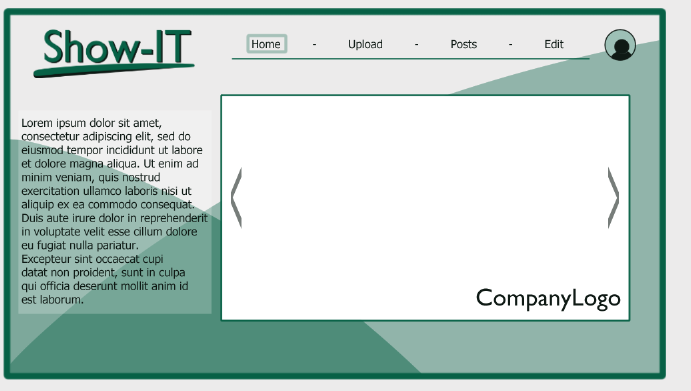
\includegraphics[scale=0.55]{1stMockup_Show-IT.png} 
        \caption{First mockup of our application.}
    \label{fig:MU}
\end{figure}

    \subsection{Mockup}
From that initial mockup we created the mockup of all the pages, with the functionality and intent for the page.
Keeping the colorscheme from the first mockup and the overall design was to be continued working with.
    See \textit {igure \ref{fig:MUA}} For the mockup of all pages.
\begin{figure} [!htbp]
    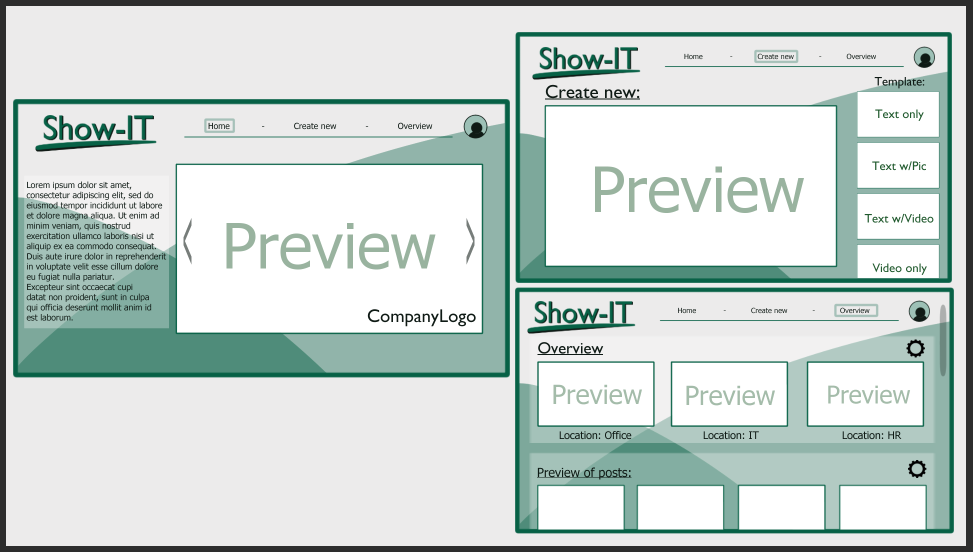
\includegraphics[scale=0.55]{mockup_all.png} 
        \caption{Mockup of all pages of applicaiton.}
    \label{fig:MUA}
\end{figure}

        \subsubsection{Home}
The home page would explain what this app is and what it does for the user, alongside a slideshow with this company's
posts or information and important things the company want to highlight.
On the home page an administrator will be able to edit what is being highlighted in the preview box. Wether it be 
company information or the same posts that are in rotation on the screens in each section of the office.

        \subsubsection{Create new}
Is an editor page that shows templates of different kinds. Sort of like "power point" editor. You can choose the template 
that fits your needs and insert what you want. These will be up to the company to create a standard. The text 
size and font will be automatic as to not create wildly different posts, and include a company logo.
This page would also be a hub for your own previously created posts, where you could pick them up from 
older archived posts or ones you have waiting and edit them.

        \subsubsection{Overview}
Here you will find an overview of the office's screen locations and what they show at this current moment as well as an
overview over the posts currently in rotation.
Here the administrators will have access to edit the posts and adjust the time they are up for as well as what will
be shown on the spesific screen locations. Only the Administrators will have access to these settings as well as 
an archive with posts that has ran its time.

    \subsection{End result}

\section{Project process}
\subsection{Methodology}
The group methodology was simple. A sprint would be created with relevant story items and some wildcard story items (Create a report...).
Certain story items were assigned to specific members, The tought was that this would ensure that everyone had atleas some managable and simple story items
to work on. When a a story item was finished a pull request would be submitted to the scrum master of the project. The scrum master would then perform
a code review before deciding if the pull request should be accepted or not. If a pull request was not accepted the story item would be moved from finished back to
in progess. The team communicated trough teams and announcements were published on scrum wise. 

\subsection{Scrum}
To manage our storyboard the team used a tool known as Scrumwise \cite*{scrumwiseScrumToolsScrum}. Scrumwise gave all team members great insight over
what tasks were beeing worked on, what tasks were reserved and what tasks were finished.

\subsection{Git\cite*{Git}}
The group utilized Git as our version control system. Each time a new commit was added to the main branch a github action would compile and publish
the applicaiton to github pages.


\pagebreak
\printbibliography

\end{document}